\section{Methodik}
\subsection{Statische Datenerfassung}

\begin{flushleft}
Die statische Datenerfassung dient dem Zweck, die Funktionalität der Wandler unter einer konstanten Last zu überprüfen. Es wurden zwei simple Testfälle aufgebaut. Bei beiden handelt es sich um Parallelschaltungen von 4,7 Ohm Widerständen. Der erste Fall schaltet zwei davon parallel, der zweite drei. Durch das Anwenden des Ohmschen Gesetzes, kann ein theoretischer Stromfluss und somit auch die theoretische Leistungsaufnahme berechnet werden. Der Wandler wird durch ein Netzteil mit 24 Volt Ausgangsspannung betrieben. Diese 24 Volt werden von dem Wandler auf 12 V herabgesetzt. 
Somit kann der Strom berechnet werden, der durch die Widerstände fließt:
\end{flushleft}



\begin{figure}
    \centering
    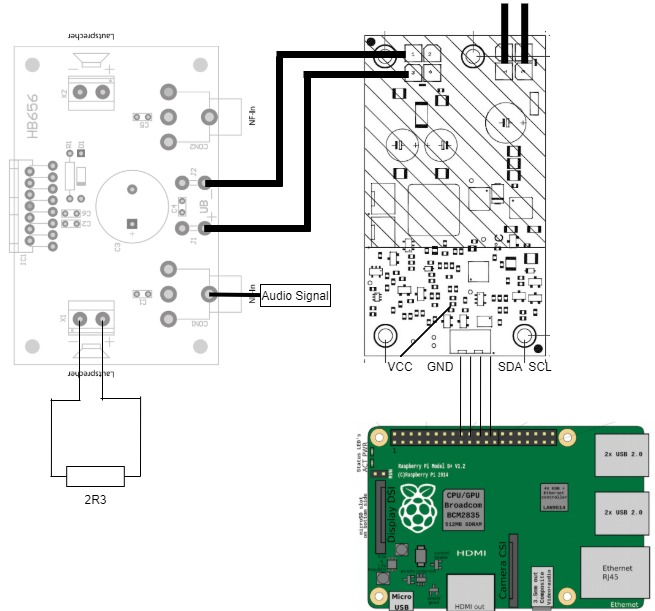
\includegraphics[height= 4cm, width = 12cm]{Pictures/Dyn_Schaltung.jpg}
    \caption{Versuchsaufbau der dynamischen Datenerfassung}
\end{figure}


\begin{equation}
\label{Ohmsches Gesetz}
\frac{U}{R} = I \tab
\end{equation}


\begin{equation}
\label{Ohmsches Gesetz}
\frac{12V}{4,7 Ohm}*2 = 5,10 A 
\frac{12V}{4,7 Ohm}*3 = 7,65 A
\end{equation}

\begin{flushleft}
Da es sich in diesen Testfällen um statische Lasten handelt, sind keine hohen Abtastraten erforderlich, deshalb wird zur Datenerfassung ein PicKit mitsamt I²C Schnittstelle verwendet und kein Raspberry Pi. 

Des Weiteren ist zu erwähnen, dass mehrere Wandler getestet wurden, einer davon mit \hl{welcher fehler}. Bei der Messung der Daten, zeigt sich, dass sowohl Temperatur als auch Ausgangsstrom, dieses Wandlers unter gleicher Last höher waren als die der anderen, was man in \hl{Abb. X erkennen kann} 
\end{flushleft}

\subsection{Dynamische Datenerfassung}
\begin{flushleft}
Das Ziel der dynamischen Datenerfassung ist es, zu evaluieren, wie der Wandler sich unter Lasten verhält, die sich mit der Zeit ändern. Sowie mögliche Abweichungen zwischen den einzelnen Wandlern selbst. Der Testaufbau beinhaltet den Hybridwandler, einen Stereoverstärker, welcher per Wandler mit Strom versorgt wird und in den ein Audiosignal eingespeist wird. Als Signal wird hierbei zu begin ein Sinussignal verwendet, welches mit dem Programm Audacity generiert wird (https://www.audacityteam.org/). Der erste Testschritt ist dabei die Überprüfung, wie hoch die maximale Frequenz eines Signals sein kann, sodass interpretierbare Daten erzeugt werden können. Die maximale Frequenz kann unter Berücksichtigung der Nyquistfrequenz theoretisch hergeleitet werden oder durch praktische Tests empirisch bestimmt werden. In Abb. 4 ist das generierte Signal zu sehen, welches in den Verstärker eingespeist wird. Dabei handelt es sich um ein 10 Hz Sinussignal. 

Das Messen der Daten erfolgt ebenfalls per I²C, jedoch auf einem Raspberry Pi, da dieser im Vergleich zum PicKit höhere Datenraten ermöglicht. Das Verarbeiten der Daten erfolgt per Python. 
\end{flushleft}

\begin{figure}
    \centering
    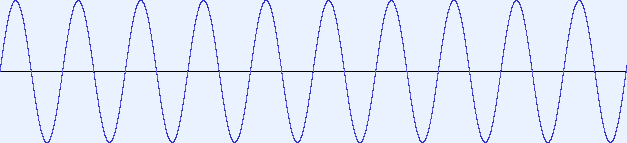
\includegraphics[height= 4cm, width = 12cm]{Pictures/Sinus_Aud.png}
    \caption{In Audacity generiertes 10 Hz Sinussignal}
\end{figure}

\begin{figure}
    \centering
    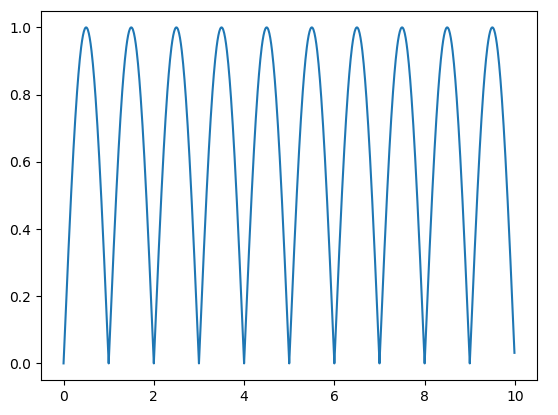
\includegraphics[height= 4cm, width = 12cm]{Pictures/Clapped_Sine.png}
    \caption{Effektive Frequenz eines 10 Hz Signals ist 20 Hz, weil, weil es für den Verstärker egal ist ob + oder - Signal }
\end{figure}

\begin{figure}
    \centering
    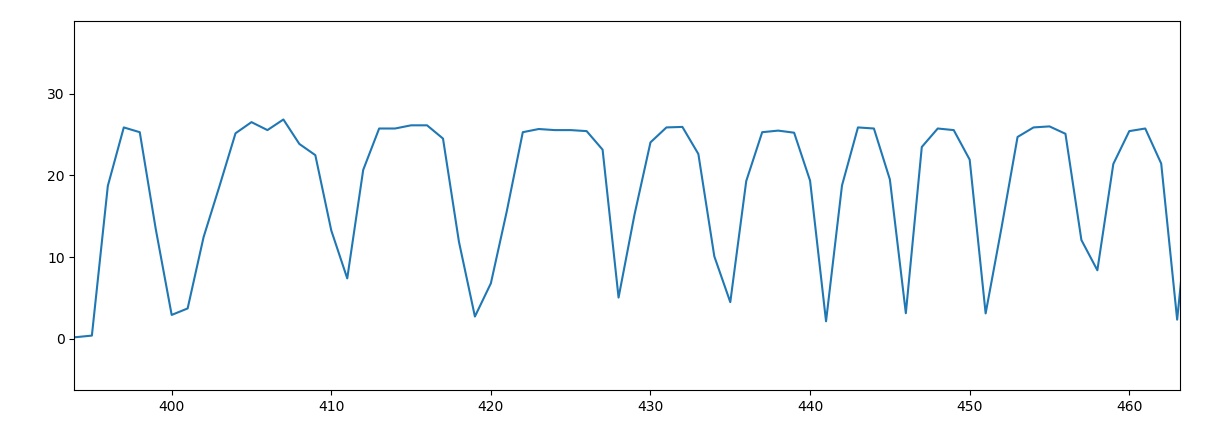
\includegraphics[height= 4cm, width = 12cm]{Pictures/TatsDaten.png}
    \caption{Tatsächlich gemessene Leistung des Wandlers}
\end{figure}

\begin{flushleft}

In Abb. 6 ist der ungefilterte Leistungsverlauf des Wandler dargestellt. Es ist ersichtlich, dass das 10 Hz Sinussignal in Abb. 5, dem gemessenen Sinussignal, entspricht. Der unsaubere Verlauf der Leistung kann auf Rauschen innerhalb der Hardware und auf die Abtastrate zurückzuführen sein. 
\end{flushleft}


\begin{equation}
\label{Sigmoid}
f\textsubscript{nyquist} = 1/2 * f\textsubscript{abtastrate}
\end{equation}

\begin{flushleft}
Die Abtastrate kann berechnet werden, da die Parameter des I²C Protokolls bekannt sind. Zeitliche Abweichungen die innerhalb des Codes entstehen sollen hier vernachlässigt werden.\hl{Es werden pro Parameter 2 Byte an Daten angefragt, somit ist pro Transfer eine Bitmenge von 1+8+1+8+1+8+1+1 = 29 bits erforderlich Bei einer Taktrate von 80 KHz ist das folglich eine Bitrate von T = 1 / 800000 = 0,0000125 s == 1 bit , -> 29 Bit = 0,0000125 *29 = 0,003625 pro Parameter *4 für alle Parameter = 0,00145 s für alle, 1/ 0,00145 = 689 Hz...} 

\hl{Experimentelle Werte zeigen, dass die maximale Abtastfrequenz bei ca. 100 Hz liegt, somit ist die Nyquistfrequenz des Signals 50Hz.}

Die linken Wert repräsentieren die Zeitstellen in Sekunden, die Rechten sind die Signaldaten, welche dann per Programm zu einer Kurve interpoliert werden. 
\end{flushleft}

\subsubsection{Echtzeitmonitoring}
Das Ziel des Echtzeitmonitoring ist es, in laufenden Betrieb Aussagen darüber zu treffen welche Last gerade an dem Wandler angeschlossen ist. Eine Last ist in diesem Fall ein Audiosignal, welches durch einen Stereo Verstärker, welcher an den Wandler angeschlossen ist, verstärkt wird.  Zur Klassifizierung, welche Last, bzw. welches Signal gerade am Stereoverstärker angeschlossen ist, wird ein neuronales Netz verwendet, welches per Tensorflow API generiert wird. Die gemessenen Signale werden dann vom Raspberry Pi per Socket an einen Rechner geschickt, welcher dann die Daten per Neuronales Netz interpretiert und eine entsprechende Klassifizierung liefert. Als Testfälle wurden Sinussignal mit verschiedenen Frequenzen verwendet, um die allgemeine Anwendbarkeit von Deep-Learning Algorithmen zu verifizieren. 




\subsubsection{Laufzeitmonitoring}

Das Ziel des Lauzeitmonitoring ist es, einen Signalverlauf aufzuzeichnen und diese Daten dann im Nachgang zu analysieren und zu Klassifizieren. 

\subsubsection{Vergleichsmonitoring mehrerer Wandler im laufenden Betrieb}

Das Ziel des Vergleichsmonitoring ist es, eine Software Struktur aufzubauen, welche es ermöglicht, mehrere Wandler gleichzeitig auf einem Raspberry Pi per I²C zu betreiben und die Daten in Echtzeit zu visualisieren und in Textdateien abzuspeichern. Dadurch, dass die verwendeten Wandler unterschiedlich Adressen besitzen, müssen keine Ergänzungen an der Schaltung durchgeführt werden, es reicht einzig die Datenleitungen (SDA, SCL) zusammenzuschalten. Während der Messung der Wandler, werden die Daten von jedem Messpunkt in Echtzeit auf ein Koordinatensystem per PyPlot übertragen. 


